\section{Introduction}\label{introduction}

Stochastic resetting---interrupting a stochastic evolution at random times and returning part of the state to a prescribed target---generically produces nonequilibrium stationary states, finite-mean first-passage times, and rich renewal structure~\cite{EvansMajumdar2011,EvansMajumdarSchehr2020}, and has been realized experimentally with holographic optical traps~\cite{TalFriedman2020,Besga2020}. In parallel, active-matter physics studies particles that convert internal energy into persistent self-propulsion~\cite{Romanczuk2012,Marchetti2013,Bechinger2016}; at finite mass the interplay of inertia, activity, and noise produces distinctive underdamped phenomenology~\cite{Lowen2020}. The intersection of the two fields is now an active frontier.

A reset clock can act on any subset of position, velocity, and orientation. Prior work has analyzed prescribed coordinate-selective resets in overdamped and inertial settings~\cite{KumarSadekarBasu,GhoshMandalChaki,Baouche,Shee,BaoucheKurzthaler2025,Gupta,Singh2020,CapalaDybiec2021,FrankeSokolov2026,OlsenLowen,Howlader2026,PatelShee}; Patel and Shee~\cite{PatelShee} identify position--velocity and velocity alone as possible protocols, anticipating distinct nonequilibrium steady-state statistics. Related work identifies upstream-sector preservation~\cite{ChakiOlsenLowen}, sorting by velocity or orientation reset~\cite{CleurenEichhorn2026}, and reset-optimized active-particle exploration~\cite{OlsenLowenCaprini2026}. Experimental implementations include optical-trap resetting~\cite{TalFriedman2020,Besga2020}; which coordinates an apparatus returns is part of the intervention. Here we compare all seven fixed-zero reset protocols within one finite-inertia model, separating changes in confinement, kinetic content and directed transport. Their exact long-time fingerprints also pose an identification question, complementary to finite-trajectory inference~\cite{FrishmanRonceray2020}.

The model has one-way sector coupling: orientation drives velocity and velocity drives position. Position reset therefore localizes the particle without changing its internal dynamics. Orientation reset can suppress or enhance kinetic content depending on the reset rate relative to inertial relaxation, whereas all four velocity-reset protocols share a kinetic trace. A tuned velocity-only/orientation-only pair has identical diffusion but different drift. These physical distinctions yield the exact decoder and the restricted-observation identities below. Coordinate-selective resetting differs from partial resetting that rescales a coordinate rather than returning it to a fixed target~\cite{TalFriedmanPartial2022}.

\section{Model and reset protocols}\label{model}

In dimensionless variables the particle obeys

\[
\begin{aligned}
d r&=v\,dt,\\
M\,dv&=-\bigl(v-\mathrm{Pe}\,u(\theta)\bigr)dt+\sqrt2\,dW_t,\\
d\theta&=\sqrt2\,dW_r,
\end{aligned}
\]

where $u=(\cos\theta,\sin\theta)$ is the self-propulsion direction, $M>0$ is the reduced mass, $\mathrm{Pe}\ge0$ the P\'eclet number, and $W_t$, $W_r$ independent Wiener processes. The dimensional scaling is $t=D_rt_d$, $r=r_d/\sqrt{D/D_r}$, $v=v_d/\sqrt{DD_r}$, $M=mD_r/\gamma$, $\mathrm{Pe}=v_a/\sqrt{DD_r}$, and $\rho=\rho_0/D_r$, with $D$ the translational and $D_r$ the rotational diffusion coefficient.

Superimposed on this evolution, an independent Poisson clock of rate $\rho>0$ triggers resets. At each event a fixed nonempty subset $q\subseteq\{P,V,\Theta\}$ of coordinates is returned deterministically to the origin of its sector: position to $r=0$, velocity to $v=0$, orientation to $\theta=0$. The seven protocols are $P,V,\Theta,PV,P\Theta,V\Theta,PV\Theta$, and we take $r(0)=v(0)=0$, $\theta(0)=0$. A protocol is thus three binary choices---reset position or not, velocity or not, orientation or not---and the question is where each choice becomes visible.

\section{Exact moment framework}\label{moment-framework}

The backward generator of the reset dynamics closes on first and second moments: means and second moments of $(r,v,u)$ obey a finite linear hierarchy that can be solved exactly for every protocol (Supplement, Secs.~S1--S3). From the solutions we extract the long-time record used throughout: stationary internal moments---the velocity matrix $S=E[vv^{\mathsf T}]$, velocity--orientation correlations, and the orientation matrix $U=E[uu^{\mathsf T}]$; stationary spatial moments for protocols that reset position; and asymptotic spatial coefficients (diffusion tensor $D$, with $D_{\mathrm{eff}}=\operatorname{Tr}D/2$, and mean drift) for protocols that do not.

One definitional point matters for everything that follows. When position is not reset, orientation resetting at $\mathrm{Pe}>0$ polarizes the propulsion direction and produces a nonzero mean velocity, hence a ballistic contribution to the raw mean-squared displacement. With position reset, the mean position instead approaches a stationary value. Centered covariance, rather than raw mean-squared displacement, defines spatial transport when orientation resetting produces drift; all spatial growth statements below refer to the centered quantity.

The hierarchy is not merely finite; it is \emph{triangular}, and that structure carries the physics. Writing $W=E[vu^\mathsf T]$, $Q=E[ru^\mathsf T]$, $C_{rv}=E[rv^\mathsf T]$, and $R=E[rr^\mathsf T]$, the moment sectors form
\[
\underbrace{(u,U)}_{\text{orientation}}\ \longrightarrow\
\underbrace{(v,W,S)}_{\text{velocity}}\ \longrightarrow\
\underbrace{(r,Q,C_{rv},R)}_{\text{position}},
\]
Orientation drives velocity through $\mathrm{Pe}\,u$, velocity drives position through $\dot r=v$, and neither coupling runs backwards. This ordering explains why position resetting leaves the internal dynamics unchanged, whereas upstream interventions can reshape downstream statistics.

The orientational decoder observable follows from a short closed balance; the full hierarchy and spatial coefficients are derived in Supplement, Secs.~S1--S3.

The orientation sector closes on itself. Orientation undergoes free rotational diffusion with generator $\partial_\theta^2$, so the second harmonic $m=E[\cos2\theta]$ obeys $\dot m=-4m$ between reset events, while an orientation reset returns $\theta$ to $0$ and hence $\cos2\theta$ to $1$ at rate $\rho$. Thus
\[
\dot m=-4m+\rho\,(1-m)
\quad\Rightarrow\quad
m_\infty=\frac{\rho}{\rho+4}
\]
when orientation is reset, and $m_\infty=0$ when it is not. Since $U_{xx}=E[\cos^2\theta]=(1+m)/2$, the two cases give $U_{xx}=(\rho+2)/(\rho+4)$ and $U_{xx}=1/2$ respectively---the orientation bit, separated by $\rho/[2(\rho+4)]>0$. This holds at every $\mathrm{Pe}$, because the orientation sector is autonomous.

\section{Coordinate-selective localization and sector invariance}\label{localization-sector-invariance}

The first fingerprint is spatial. Define the growth class $G(q)$ of protocol $q$ as \emph{localized} if the centered spatial covariance $\operatorname{Cov}(r(t))$ has a finite limit and \emph{diffusive} if it grows linearly. Then, within the seven-protocol family, position reset is an exact localization switch:

\[
G(q)=\text{localized}\iff P\in q .
\]

If $P\in q$, the resolvent structure of the reset generator yields a finite stationary centered covariance in closed form. If $P\notin q$, then $\operatorname{Cov}(r(t))=2Dt+O(1)$ with $D\succ0$ at every fixed finite parameter point: both diagonal entries are strictly positive for $M>0$, $\rho>0$, and $\mathrm{Pe}\ge0$ (Supplement, Sec.~S3.2), whatever the reset protocol does to velocity and orientation. There is no intermediate case, no parameter window of anomalous growth, and no exception at special $(M,\rho,\mathrm{Pe})$.

The second fingerprint is what the switch does \emph{not} do. Position is a downstream coordinate: it integrates velocity but feeds back on nothing. Resetting it therefore cannot influence the internal $(v,u)$ dynamics, and the three position-toggle pairs satisfy exact internal-sector identities

\[
PV\equiv V,\qquad P\Theta\equiv\Theta,\qquad PV\Theta\equiv V\Theta
\]

on the full internal $(v,u)$ process, including higher statistics (Supplement, Sec.~S5.1). An analogous upstream-marginal preservation was observed for unidirectionally coupled passive coordinates~\cite{ChakiOlsenLowen}. Here a localized cloud and a spreading particle have identical internal dynamics: position reset localizes motion without changing kinetic energy, orientational order, or velocity--orientation correlations.

Velocity and orientation resets, by contrast, act upstream and reshape the internal state itself: orientation reset polarizes $u$ and, when position is not reset, drives a mean drift at $\mathrm{Pe}>0$, while velocity reset drains kinetic energy. These are the fingerprints the decoder reads next.

\section{Observable fingerprints and the exact protocol decoder}\label{decoder}

Collect three long-time observables into the signature

\[
\Sigma(q)=(G(q),U_{xx}(q),\operatorname{Tr}S(q)).
\]

\textbf{Theorem (three-observable decoder).} For every fixed $M>0$, $\rho>0$, and $\mathrm{Pe}\ge0$, the map $q\mapsto\Sigma(q)$ is injective on the seven nonempty reset protocols: the signature exactly decodes all seven protocols.

The proof is a three-branch argument (Supplement, Secs.~S3--S4), and each branch reads one bit. The growth class $G$ reads the position bit, by the localization switch above. The orientational moment $U_{xx}$ reads the orientation bit, by the autonomous balance of Sec.~\ref{moment-framework}: free rotational diffusion isotropizes the orientation to $1/2$, while resetting to $\theta=0$ sustains excess alignment at $(\rho+2)/(\rho+4)$, a gap of $\rho/[2(\rho+4)]>0$ that persists at every $\mathrm{Pe}$. Once these two bits are fixed, the only remaining ambiguity is the velocity bit within each class---$P$ versus $PV$, $P\Theta$ versus $PV\Theta$, $\Theta$ versus $V\Theta$. Here the kinetic trace is described by three expressions across the seven protocols; the first and third can coincide. Writing $D_\star=M\rho+M+1$, each splits into a thermal and an activity contribution:
\[
\begin{aligned}
A&=\operatorname{Tr}S_P=\frac{2}{M}+\frac{\mathrm{Pe}^2}{M+1},\\[3pt]
B&=\operatorname{Tr}S_{PV}=\operatorname{Tr}S_{V}=\operatorname{Tr}S_{PV\Theta}=\operatorname{Tr}S_{V\Theta}\\[1pt]
&=\frac{4}{M(M\rho+2)}+\frac{2\mathrm{Pe}^2}{(M\rho+2)D_\star},\\[3pt]
C&=\operatorname{Tr}S_{P\Theta}=\operatorname{Tr}S_{\Theta}
=\frac{2}{M}+\frac{\mathrm{Pe}^2\bigl(M\rho^2+\rho+1\bigr)}{(\rho+1)D_\star}.
\end{aligned}
\]
The free value $A$ is the $d=2$ specialization of Eq.~(14) of Patel and Chaudhuri~\cite{PatelChaudhuri2023}; the complete-reset value $B$ is Eq.~(5) of Patel and Shee~\cite{PatelShee}, here extended to all four velocity-reset protocols. For the velocity-retaining protocols, with $\Sigma_u=\operatorname{Cov}(u)$, the exact kinetic trace separates into velocity fluctuations and induced mean propulsion:
\[
\operatorname{Tr}S_{\Theta}=\frac{2}{M}+\frac{\mathrm{Pe}^2\operatorname{Tr}\Sigma_u}{1+M(1+\rho)}+|\bar v|^2,
\qquad
\operatorname{Tr}\Sigma_u=\frac{1+2\rho}{(1+\rho)^2},
\qquad
|\bar v|=\frac{\mathrm{Pe}\rho}{1+\rho}.
\]
Subtracting the free trace $2/M+\mathrm{Pe}^2/(1+M)$ gives
\[
C-A=\frac{\mathrm{Pe}^2M\rho(M\rho-1)}{(1+M)(1+\rho)D_\star}.
\]
Orientation reset reduces orientational fluctuations and increases their relaxation rate from $1$ to $1+\rho$, reducing the activity-driven velocity fluctuations, but it also induces mean propulsion. For positive activity these effects balance at $M\rho=1$: $C<A$ below resonance and $C>A$ above it. This competition concerns only velocity-retaining protocols; all four velocity-reset protocols share the complete-reset kinetic trace $B$, independently of orientation reset.

The three velocity pairs are therefore separated by two gaps, each with a strictly positive thermal term and a nonnegative activity term:
\[
\begin{aligned}
A-B&=\frac{2\rho}{M\rho+2}
+\frac{M\rho\,\mathrm{Pe}^2\bigl(M\rho+M+3\bigr)}{(M+1)(M\rho+2)D_\star},\\[3pt]
C-B&=\frac{2\rho}{M\rho+2}
+\frac{M\rho\,\mathrm{Pe}^2\bigl(M\rho^2+3\rho+1\bigr)}{(\rho+1)(M\rho+2)D_\star}.
\end{aligned}
\]
Both gaps are thus at least the common thermal floor $2\rho/(M\rho+2)>0$ at every point of the domain---the common passive-point gap---while the activity terms are nonnegative and are strictly positive whenever $\mathrm{Pe}>0$. Positivity is therefore immediate by inspection, with no cancellation to check. This completes the proof: $G$ fixes the position bit, $U_{xx}$ the orientation bit, and the two positive gaps resolve the velocity bit in every remaining case. Table~\ref{tab:decoder} displays the branch values.

The decoder uses a categorical growth class and two scalar moments.

\begin{table}[t]
\tbl{Exact matched-parameter decoder signature. $G$ is categorical.\label{tab:decoder}}
{\begin{tabular}{c|c|c|c}
Protocol & $G$ & $U_{xx}$ & $\operatorname{Tr}S$\\ \hline
$P$ & localized & $1/2$ & $A$\\
$V$ & diffusive & $1/2$ & $B$\\
$\Theta$ & diffusive & $(\rho+2)/(\rho+4)$ & $C$\\
$PV$ & localized & $1/2$ & $B$\\
$P\Theta$ & localized & $(\rho+2)/(\rho+4)$ & $C$\\
$V\Theta$ & diffusive & $(\rho+2)/(\rho+4)$ & $B$\\
$PV\Theta$ & localized & $(\rho+2)/(\rho+4)$ & $B$
\end{tabular}}
\end{table}

Figure~\ref{fig:transport} gives representative transport and localization curves before we turn to the information discarded by restricted records.

\begin{figure}[!t]
\centering
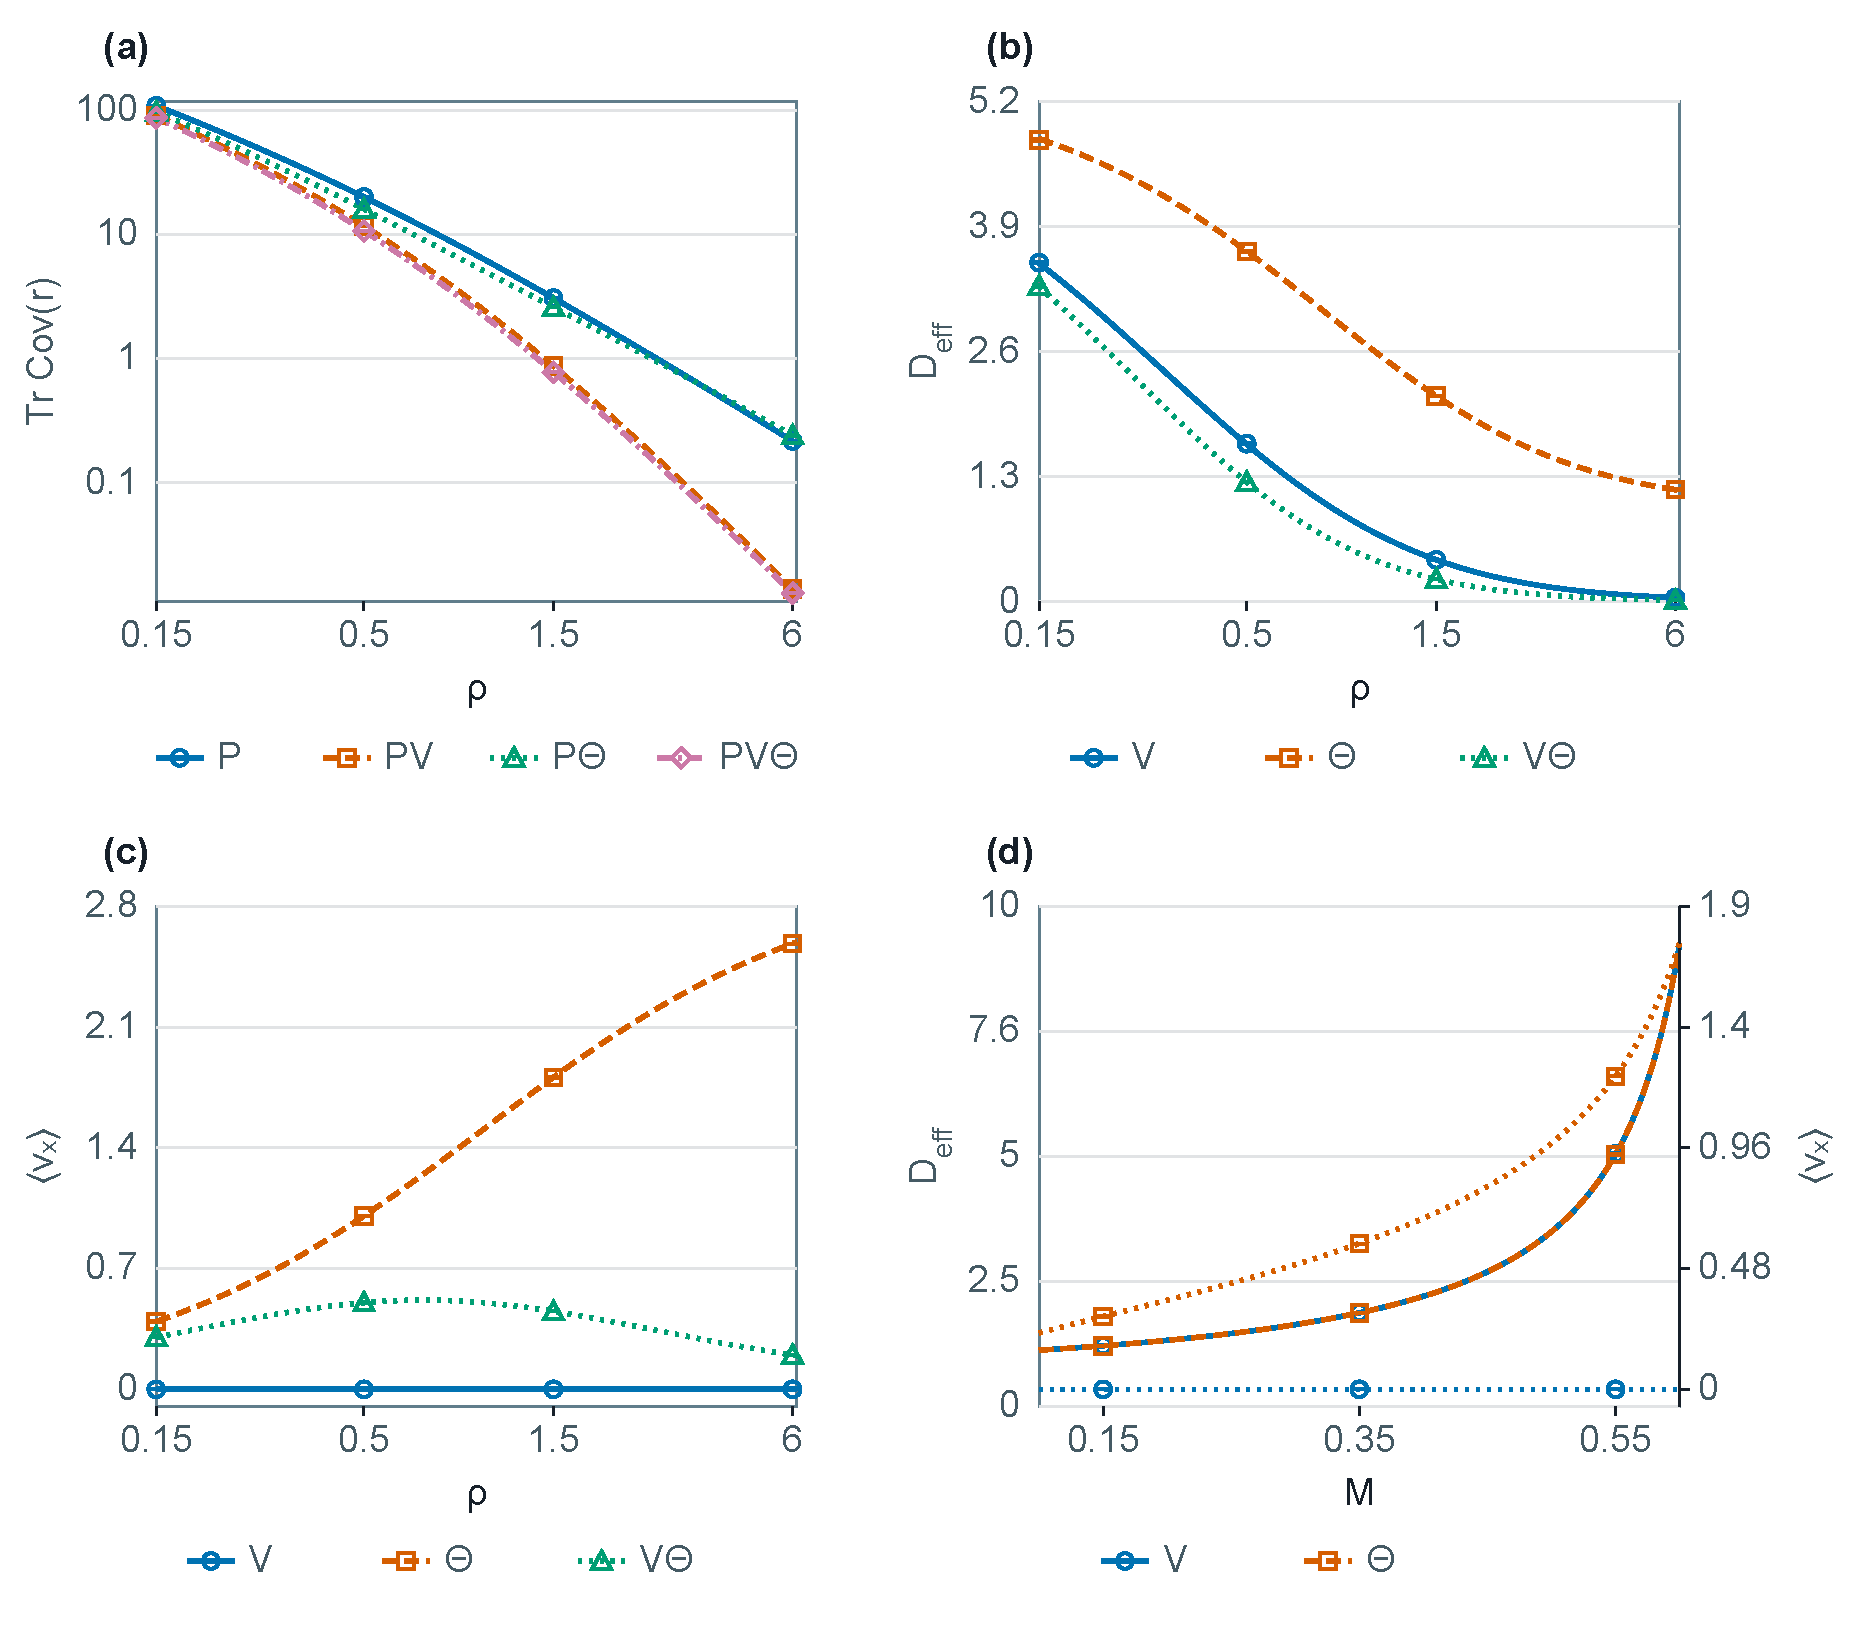
\includegraphics[width=0.82\textwidth]{../../../figures/F-080-transport-localization.pdf}
\caption{Exact transport and localization. Panels (a)--(c) use $M=2$ and $\mathrm{Pe}=3$: (a)~stationary centered variance of the four localized protocols; (b)~centered effective diffusion of the three diffusive protocols; (c)~mean drift along the reset direction, zero for $V$ and finite for $\Theta$ and $V\Theta$. Panel (d) uses $\rho=1/2$ along the stated $\mathrm{Pe}(M)$ curve: the diffusion coefficient (left axis) coincides for $V$ and $\Theta$, while the dotted mean drift (right axis) separates them. Curves are exact; symbols are paired Richardson estimates from independent trajectories with one-SE bars (bars smaller than a symbol may be obscured). Rate axes in (a)-(c) and the variance axis in (a) are logarithmic. Full numerical results and precision details are given in Table S1.}
\label{fig:transport}
\end{figure}
\FloatBarrier

\section{Information loss under restricted observation}\label{information-loss}

At matched parameters, protocols are $\mathcal O$-equivalent when all observables in $\mathcal O$ agree. Table~\ref{tab:subsignatures} gives the exact classes for proper sub-signatures; Supplement Sec.~S5 covers the second-order record. Three mechanisms explain the lost information.

\begin{table}[t]
\tbl{Numbers of distinguishable classes. $T=\operatorname{Tr}S$; the exceptional set is $\mathrm{Pe}=0$ or $M\rho=1$.\label{tab:subsignatures}}
{\begin{tabular}{lcc}
\toprule
Retained record & Generic & Exceptional\\
\midrule
$G$ & 2 & 2\\
$U_{xx}$ & 2 & 2\\
$T$ & 3 & 2\\
$(G,U_{xx})$ & 4 & 4\\
$(G,T)$ & 5 & 4\\
$(U_{xx},T)$ & 4 & 4\\
$\Sigma=(G,U_{xx},T)$ & 7 & 7\\
\botrule
\end{tabular}}
\end{table}

\emph{Internal observations hide position reset.} By sector invariance, the entire internal record---every function of $(v,u)$---is blind to the position bit: under internal observation the seven protocols collapse to the four classes $\{P\},\{V,PV\},\{\Theta,P\Theta\},\{V\Theta,PV\Theta\}$. An experiment that tracks speed and orientation but not displacement cannot tell a localized system from a transporting one.

\emph{Scalar traces hide orientation structure.} Contracting matrices to traces discards the anisotropy that stores the orientation bit. For $PV/PV\Theta$ the scalar triple $(\operatorname{Tr}S,\operatorname{Tr}C_{rv},\operatorname{Tr}R)$ agrees exactly---a consequence of $\operatorname{Tr}U=1$---although for finite activity the centered spatial variances differ by the explicit gap $\mathrm{Pe}^2/[(1+\rho)^2(1+M\rho)^2]$, which is strictly positive for $\mathrm{Pe}>0$ and vanishes at the passive point. Likewise $\operatorname{Tr}S_V=\operatorname{Tr}S_{V\Theta}$ at every finite parameter point, while orientational moments and drift separate the pair. Thus scalar traces can hide orientation information that remains visible in orientational moments.

\emph{Parameter-specific observational coincidences.} The trace triple for $P/P\Theta$ differs by terms proportional to $\mathrm{Pe}^2(M\rho-1)$, so it coincides on the resonance $M\rho=1$---where the reset rate matches the velocity relaxation rate---and at the passive point $\mathrm{Pe}=0$. The two coincidences are resolved differently. On the resonance, activity is still present and both the orientational mean $\bar u_x$ and the positional mean $\bar r_x=\mathrm{Pe}/(1+\rho)$ separate the pair. At $\mathrm{Pe}=0$ the entire translational sector of $P$ and $P\Theta$ coincides---in particular $\bar r_x=0$ for both---and only orientational observables such as $\bar u_x=\rho/(1+\rho)$ remain as witnesses. The same passive coincidence pairs $PV/PV\Theta$ and $V/V\Theta$, since without propulsion the orientation no longer couples to motion; orientational observables keep every such pair distinct for all $\rho>0$. At this passive endpoint, $D_\Theta=I$ for every $\rho>0$. For $\mathrm{Pe}>0$ and $\rho>0$, the anisotropy is $D_{\Theta,xx}-D_{\Theta,yy}=-\mathrm{Pe}^2\rho(2\rho-1)/[(1+\rho)^3(4+\rho)]$. These orientation-only coefficients recover the overdamped orientation-reset result of Kumar, Sadekar and Basu~\cite{KumarSadekarBasu}, Eq.~(46); with velocity retained, translational inertia leaves their long-time values unchanged. Here they enter the exact comparison with velocity-reset transport. Thus $D_\Theta$ is isotropic only at $\rho=1/2$.

The sign change is a centered effect: $\Sigma_{u,xx}-\Sigma_{u,yy}=\rho/(\rho+4)-\rho^2/(1+\rho)^2=\rho(1-2\rho)/[(\rho+4)(1+\rho)^2]$, and $D_\Theta$ carries this difference times $\mathrm{Pe}^2/(1+\rho)$. Thus at $\rho=1/2$ centered spreading is isotropic despite nonzero polarization; isotropic covariance does not imply an isotropic orientation distribution.

Since $D_V$ is isotropic, $D_\Theta=D_V$ can occur only there; on that line tensor equality reduces to one scalar equation for $\mathrm{Pe}^2(M)$,

\[
\begin{gathered}
\rho=\tfrac12,\qquad 0<M<M_\star\approx0.658,\\[2pt]
\mathrm{Pe}^2=\frac{27M(M+6)(3M+2)}{2\,(44-9M-80M^2-12M^3)},
\end{gathered}
\]


on which velocity-only and orientation-only resetting share the same centered effective diffusion tensor: two entirely different microscopic interventions---draining kinetic energy versus re-aligning propulsion---produce identical spatial spreading. The coincidence is broken by the mean drift, which vanishes for $V$ and is nonzero for $\Theta$ at $\mathrm{Pe}>0$.

\section{Representative parameter dependence}\label{parameter-dependence}

Figure~\ref{fig:transport} compares localization, diffusion and drift. Resetting velocity accelerates the high-rate localization decay because each interval starts from rest. Drift separates the tuned $V/\Theta$ diffusion coincidence in panel~(d). The limits $M\to0^+$ and $\rho\to0^+$ are singular boundaries of the fixed-finite-parameter classification (Supplement, Sec.~S6).

For the localized protocols, the stationary centered variance decreases with reset rate at the plotted parameters. In the frequent-reset limit, retaining velocity gives $\rho^2E_P|r|^2\to4/M+2\mathrm{Pe}^2/(1+M)$, whereas resetting velocity gives $\rho^3E_{PV}|r|^2\to8/M^2$. For diffusive protocols, $D_{\mathrm{eff},V}\sim(\mathrm{Pe}^2+4)/(2M^2\rho^2)$ at high rate, while $D_{\mathrm{eff},\Theta}\to1$ and $\bar v_\Theta\to\mathrm{Pe}\,e_x$. Thus velocity reset acts as a transport brake, whereas orientation reset polarizes propulsion; the $V\Theta$ drift decays as $\mathrm{Pe}/(M\rho)$.

\begin{samepage}
After inspection of the finest-step results, Richardson extrapolation was adopted using the existing coupled paths without new sampling (Supplement, Sec.~S0.2). The raw-finest analysis already contained 80/80 intervals, with 0 contradicted and 78/80 meeting the stricter target; its $\operatorname{Tr}S$ residuals reached about $+8.1$ SE. Kinetic-trace convergence ratios were 1.999--2.006, and Richardson did not rescue containment. Table~S1 reports the paired combinations $2X_h-X_{2h}$, which cancel the leading $O(h)$ bias; scale-normalized SEs are below 1\%, and raw finest-step values are archived.
\par\end{samepage}

\section{Discussion and conclusion}\label{discussion}

Position resetting can localize a particle while leaving its complete internal dynamics unchanged. For velocity-retaining protocols, orientation resetting changes alignment and kinetic content, with suppression below $M\rho=1$ and enhancement above it at positive activity; velocity resetting suppresses transport and gives the same kinetic trace across four protocols. The tuned $V/\Theta$ coincidence shows why matching diffusion alone does not identify the intervention: equal spreading can coexist with different drift. The three-observable decoder is a compact consequence of these sector distinctions, while its proper sub-signatures quantify exactly which distinctions a restricted measurement loses.

The moment statements follow exactly from the deterministic hierarchy, and internal-sector invariance follows from the reset generator. The theorem is restricted to fixed zero targets, matched $M>0$, $\rho>0$, and $\mathrm{Pe}\ge0$, rather than finite-data inference, singular limits, or changed targets. The theorem does not exclude a different two-observable family. The independent grid calculation reproduces selected moment formulas at prespecified points; it does not establish the full theorem set.

\section{Data and code availability}\label{data-and-code-availability}

The R6B manuscript sources, reproducibility code (software version 3.2.0rc2), and numerical records are available at Zenodo, DOI: \href{https://doi.org/10.5281/zenodo.22924890}{10.5281/zenodo.22924890}.
